\section{Motivating Example}
\label{sec:exmpl}

\begin{figure}[t]
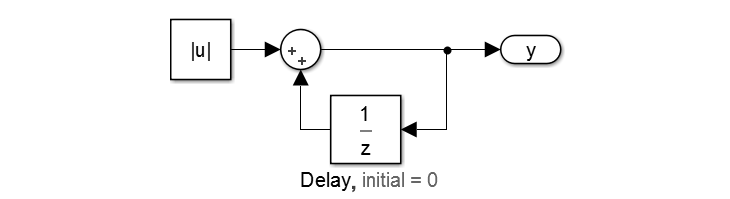
\includegraphics[width=\columnwidth]{figs/simulink-ivc.png}
{\smaller
\begin{verbatim}
node filter(x, a : real) returns (b, y : real);
let
  b = if a >= 0.0 then a else -a;
  y = b + (0.0 -> pre y);
tel;
\end{verbatim}
}
\caption{Model with property $y \geq 0$, after IVC analysis}
\label{fig:ex-after}
\end{figure}

Consider the model shown both graphically and textually in
Figure~\ref{fig:ex-before}. This model takes an input, combines it
with the previous output in some way, takes the absolute value, and
then adds this to an accumulating value. This model has the property
that the output is always non-negative, i.e., $y \geq 0$. Moreover, it
happens that this property holds regardless of the way the input is
combined with the previous output, i.e., the function $f$ in the
model. Formally, we say that the inductive validity core (IVC) does
not contain that part of the model. The model reduced to its IVC is
shown in Figure~\ref{fig:ex-after}. Note that most static dependency
analyses would not be able to remove $f$ from the model.

%% \begin{itemize}
%%     \item Not sure if this should go before or after the background section with a description of Lustre.
%%     \item Need a small but interesting example.  Andrew, do any of the models that you use as jkind tests
%%         function in this way?  It would be nice to look at what we have lying around; we need something 
%%         that requires invariants.
%%     \item It would also be good to have a few points of interest with the model-requirement pairing: 
%%     \item \quad   vacuity due to an overconstrained environment 
%%     \item \quad   definitions within the model that are irrelevant to the proof.
%%     \item Explain the model and the proof process.
%% \end{itemize}
